% This is samplepaper.tex, a sample chapter demonstrating the
% LLNCS macro package for Springer Computer Science proceedings;
% Version 2.20 of 2017/10/04
%
\PassOptionsToPackage{unicode}{hyperref}
\PassOptionsToPackage{hyphens}{url}

\documentclass[runningheads]{llncs}
%
\usepackage{fixltx2e}
\usepackage[american]{babel}
\usepackage[utf8]{inputenc}
\usepackage{csquotes}
\usepackage{graphicx}
\usepackage{xcolor}
\usepackage{hyperref}
\usepackage{url}
\usepackage[T1]{fontenc}
\usepackage{lmodern}
\usepackage{microtype}
\usepackage{eurosym}
\usepackage{biblatex}
%\usepackage{float}
%\usepackage{ragged2e}
%\usepackage{tabularx}
\usepackage{caption}
%\usepackage{ulem}
\addbibresource{bibliography.bib}
\addbibresource{rpackages.bib}


% Used for displaying a sample figure. If possible, figure files should
% be included in EPS format.
%
% If you use the hyperref package, please uncomment the following line
% to display URLs in blue roman font according to Springer's eBook style:
%\renewcommand\UrlFont{\color{blue}\rmfamily}
\hypersetup{breaklinks=true,
            bookmarks=true,
            pdfauthor={},
            pdftitle={Defend Your Enemy. A Qualitative Study on Defending Political Opponents Against Hate Speech Online},
            colorlinks=true,
            citecolor=blue,
            urlcolor=blue,
            linkcolor=magenta,
            pdfborder={0 0 0}}
\urlstyle{same}


\usepackage{booktabs}
\usepackage{longtable}
\usepackage{array}
\usepackage{multirow}
\usepackage{wrapfig}
\usepackage{float}
\usepackage{colortbl}
\usepackage{pdflscape}
\usepackage{tabu}
\usepackage{threeparttable}
\usepackage{threeparttablex}
\usepackage[normalem]{ulem}
\usepackage{makecell}
\usepackage{xcolor}
\usepackage{longtable,booktabs}
\newcommand{\eg}{e.\,g.,\ }
\newcommand{\ie}{i.\,e.,\ }
%\setkeys{Gin}{width=\maxwidth,height=\maxheight,keepaspectratio}

\IfFileExists{upquote.sty}{\usepackage{upquote}}{}
% use microtype if available
\IfFileExists{microtype.sty}{%
\usepackage{microtype}
\UseMicrotypeSet[protrusion]{basicmath} % disable protrusion for tt fonts
}{}

\providecommand{\tightlist}{%
  \setlength{\itemsep}{0pt}\setlength{\parskip}{0pt}}

\begin{document}
%
\title{Defend Your Enemy. A Qualitative Study on Defending Political Opponents Against Hate Speech Online}
%

\titlerunning{Defend Your Enemy Against Hate Speech}

% If the paper title is too long for the running head, you can set
% an abbreviated paper title here
%
\author{Lilian Kojan\inst{1}\orcidID{0000-0002-4064-4447} \and
Hava Melike Osmanbeyoglu\inst{2} \and
Laura Burbach\inst{1}\orcidID{0000-0001-6233-3116}
Martina Ziefle\inst{1}\orcidID{0000-0002-6105-4729}\and
André Calero Valdez\inst{1}\orcidID{0000-0002-6214-1461}}
%
\authorrunning{L. Kojan et al.}
% First names are abbreviated in the running head.
% If there are more than two authors, 'et al.' is used.
%
\institute{Human-Computer Interaction Center, RWTH Aachen University, Campus Boulevard 57, 52076 Aachen, Germany\\
\email{\{kojan,burbach,ziefle,calero-valdez\}@comm.rwth-aachen.de}\and
RWTH Aachen Univeristy, Templergraben 44, 52052 Aachen, Germany
\email{melike.osmanbeyoglu@rwth-aachen.de}}
%


%
\maketitle              % typeset the header of the contribution
%
\begin{abstract}
Both hate speech and disinformation negatively influence the internet's potential for public deliberation and lead to polarization between political groups. In this paper, we examine the potential of counter speech to bolster public deliberation and reduce polarization. In two focus groups, we interview participants on what motivates them to engage in counter speech in general as well as counter speech favoring political adversaries. Firstly, we find a sharp distinction between participants who avoid engaging with hate speech and participants who actively engage with hate speech in order to combat it. Thus, the most important predictor for counter speech favoring adversaries is an individual's propensity for counter speech in general. In turn, motivations for counter speech in general are a strong sense of morality, a perception of the internet as an important space for public deliberation, and a sense of responsibility to enforce rules for a fair debate. Many of those participants view their online activitiy as a form of activism. Additionally, individuals engaging in counter speech hope to positively influence not necessarily the hater, but the broader audience.

	\keywords{Hate Speech \and Counter Speech \and Social Media \and Political Deliberation}
\end{abstract}
%
%
%
\Urlmuskip=0mu plus 1mu
\setcounter{footnote}{0}

\hypertarget{deliberation-in-digital-media}{%
\section{Deliberation in Digital Media}\label{deliberation-in-digital-media}}

Since the commercialization of the Internet, the relationship between digital media and political life has grown ever stronger \autocite{boulianneTwentyYearsDigital2018}.
Apart from election campaigns, one important facet is the Internet's potential to strengthen democratic society by facilitating public deliberation \autocite{papacharissiVirtualSphereInternet2002,chenOnlineIncivilityPublic2017}.
At the same time, several limitations for online public deliberation have emerged.
For one, offline power imbalances are often mirrored in the online world through an overrepresentation of groups in power, e.g., well-educated white men \autocite{feezellPredictingOnlinePolitical2016}. In addition, online groups tend to be very homogenous meaning that users are seldomly exposed to cross-cutting opinions or differing viewpoints \autocite{colleoniEchoChamberPublic2014}. And when differing opinions do collide, incivility and even hate speech can occur \autocite{papacharissiDemocracyOnlineCivility2004,coeOnlineUncivilPatterns2014,rainsIncivilityPoliticalIdentity2017}.

\hypertarget{hate-speech-and-misinformation}{%
\subsection{Hate Speech and Misinformation}\label{hate-speech-and-misinformation}}

Although hate speech has been extensively discussed by the public at large as well as studied in academia, finding an universally valid definition is challenging \autocite{gagliardoneCounteringOnlineHate2015}. Legal institutions and social networks alike tend to provide broad definitions that allow for judgement and possible sanctions on a case-by-case basis \autocite{gagliardoneCounteringOnlineHate2015}.

From a communication science perspective, \textcite{erjavecYouDonUnderstand2012} define hate speech as an expression that is in itself harmful or possibly harm-inciting and targets members of a group determined by characteristics like race or sexual orientation. Similar characteristics can be found in other definitions that consider the purpose and the effects of hate speech. \textcite{waldronHarmHateSpeech2012} characterizes speech as hateful when it serves one or both of two functions: Firstly, to dehumanize a target group and diminish its members and secondly, to reinforce a sense of in-group with other like-minded individuals. Similarly, Susan Benesch has coined the term \emph{dangerous speech} which she defines as \enquote{{[}a{]}ny form of expression (e.g.~speech, text, or images) that can increase the risk that its audience will condone or commit violence against members of another group.} \autocite{beneschDangerousSpeechPractical2020} Often, the groups targeted are marginalized social groups \autocite{alvarez-benjumeaNormativeChangeCulture2018}. But especially in common parlance, hate speech can also describe speech directed at groups like politicians that are arguably powerful \autocite{gagliardoneCounteringOnlineHate2015}. In summary, hate speech both reenforces the boundaries between groups and is harmful to members of the other group, either in itself or in its effects.

Hate speech is inextricably linked to disinformation. For one, online hate often takes the form of over-generalization, exaggeration or even outright deceit about the targeted group. E.g., \textcite{awanIslamophobiaSocialMedia2016} stresses the use of false stories to exacerbate islamophobic hate. For another, disinformation like fake news often serve the same purpose as hate speech: Polarization, radicalization and othering of the out-group \autocite{bennettDisinformationOrderDisruptive2018}.

There is ample evidence for the damaging effects of hate speech, not only on the victim of the hate speech but also on the broader audience.
Constant exposition shapes the users worldview and influences their decision-making \autocite{jubanyBackgroundsExperiencesResponses2016,erjavecReadersOnlineNews2014}.
Reading hateful and uncivil content increases attitude polarization \autocite{borahDoesItMatter2014,kimIncivilityFacebookPolitical2019}.
And by inducing negative emotions, it can also discourage people from engaging in discourse \autocite{hwangDoesCivilityMatter22,hwangSeeingBelievingEffects2014,kimIncivilityFacebookPolitical2019,molinaRoleCivilityMetacommunication2018}. Thereby, it actively impedes on the Internet's potential for public deliberation.

One possible way to counter hate speech is counter speech. Counter speech can be defined as a dissenting response to hate speech \autocite{wrightVectorsCounterspeechTwitter2017}.
Although it is sometimes used in a way that also encompasses actions like flagging hateful content, our study focusses on counter speech in the form of content, e.g., comments in answer to the hateful content itself.

\hypertarget{effectiveness-of-counter-speech}{%
\subsection{Effectiveness of Counter Speech}\label{effectiveness-of-counter-speech}}

Counter speaking is encouraged in many anti-hate speech programs \autocite{gagliardoneCounteringOnlineHate2015}. Furthermore, \textcite{chenOnlineIncivilityPublic2017} argues that countering online incivility is necessary to realize the potential of online spaces as a place for political deliberation. In spite of that, only a few studies have actually evaluated the effectiveness of counter speech. \textcite{buergerCounterspeechLiteratureReview2019} have reviewed the studies available in November 2019. They differentiate between the effects of counter speech on the hateful speaker and the effects on the wider audience.

The results oncerning the effects of counter speech on the hateful speaker are inconclusive \autocite{buergerCounterspeechLiteratureReview2019}. However, there is some evidence that counter speech by users that are perceived as more influential, can curb hate speech at least temporarily (e.g., \autocite{mungerTweetmentEffectsTweeted2017}). Findings on the effects of counter speech on the wider audience are less ambiguous. They all find evidence for something that \textcite{buergerCounterspeechLiteratureReview2019} call the \enquote{contagion effect}, i.e., the presence of hateful comments increases the probability of a user also making a hateful comment. On the opposite hand, civil comments also lead to more civil comments. Moreover, meta-comments urging people to be civil promote further meta-comments about discussion quality \autocite{molinaRoleCivilityMetacommunication2018}.

So while further research on the effects of counter speech is desirable, the existing indications for its success prompts us to ask what predicts users engaging in counter speech.

\hypertarget{predictors-for-counter-speech}{%
\subsection{Predictors for Counter Speech}\label{predictors-for-counter-speech}}

There already exist several studies examining willingness to intervene against hate speech and incivility in general and even more studies from the field of cyber-bystander research. As bystander intervention in cyber-bullying is similar to counter speech, predictors from a review on cyber-bystanding studies by \textcite{lambeStandingBullyingSocial2019} are included as well.

The following predictors refer to intervention intention, with intervention ranging from more distanced behavior like using the reporting function (e.g., \autocite{wongCombatingOnlineAbuse2016}) to deeply involved behavior like verbally confronting the individual engaging in hate speech (e.g., \autocite{dickterConfrontNotConfront2013}).

The factors we summarize as \emph{individual factors} concern properties of a would-be counter speaker that make intervention more likely. The predictors found are female gender \autocite{lambeStandingBullyingSocial2019,wilhelmGenderedMoralityBacklash2019}, high prosociality and empathy \autocite{lambeStandingBullyingSocial2019}, high self-efficacy \autocite{lambeStandingBullyingSocial2019}, a negative attitude towards passive bystanding \autocite{lambeStandingBullyingSocial2019}, an expectation that defending will help \autocite{lambeStandingBullyingSocial2019}, and a high importance of morality, including low moral disengagement, high moral identity scores and individualizing moral foundation \autocite{lambeStandingBullyingSocial2019,wilhelmGenderedMoralityBacklash2019}. Additionally, there are situation-dependent factors like the would-be counter speaker feeling negative affect \autocite{chenOnlineIncivilityPublic2017,dickterConfrontingHateHeterosexuals2012,dickterConfrontNotConfront2013} and them perceiving social pressure and responsibility to intervene \autocite{dickterConfrontingHateHeterosexuals2012,dickterConfrontNotConfront2013,wongCombatingOnlineAbuse2016}.

Other factors relate to the \emph{properties of the victim} of the hate speech or bullying. Users are more likely to intervene if the victim is an individual person as a victim rather than an abstract social group \autocite{naabFlaggingUncivilUser2018}, if the victim is more popular \autocite{lambeStandingBullyingSocial2019}, if they have a friendship or positive relationship with the victim \autocite{lambeStandingBullyingSocial2019} and if they exhibit a low level of prejudice towards the victims's social group \autocite{dickterConfrontingHateHeterosexuals2012}.

Concerning \emph{situational factors}, users were more likely to intervene if the situation was more deviant \autocite{dickterConfrontingHateHeterosexuals2012,dickterConfrontNotConfront2013,naabFlaggingUncivilUser2018}, if there was more than one perpetrator \autocite{kazerooniCyberbullyingBystanderIntervention2018} and if more steps of the bystander intervention model were met (situation is noticed, fewer number of bystanders, information on how to confront is provided) \autocite{lambeStandingBullyingSocial2019,naabFlaggingUncivilUser2018}.

To summarize, the existing research on hate speech intervention mainly considers the properties of the would-be counter speaker. For this study, we wanted to further the research on hate speech intervention by focussing in on the relationships between the would-be counter speaker and the victim. To be precise, with hate speech as an instrument for social division and polarization, can counter~speech bridge the gap between in- and out-group? Therefore, our research question is:

\emph{In social media discussions, what are predictors for users to engage in counter speech in support of political adversaries?}

\hypertarget{method}{%
\section{Method}\label{method}}

As laid out in chapter \ref{predictors-for-counter-speech}, there is some research on predictors for counter speech in general as well as a breadth of studies in the field of cyber-bystander research. To our knowledge, however, there have not been any studies on out-group favoring counter speech. Therefore, an exploratoy study design was chosen. Data was gathered in two focus groups. Afterwards, the data was transcribed and analysed to find the most pertinent predictors. The full transcriptions and the full analysis as well as the questionnaire, the slides and the guide used to collect our data can be found in our github repository for this project.\footnote{The repo can be found here: (\href{http://github.com/digitalemuendigkeit/misdoom2020}{github.com/digitalemuendigkeit/misdoom2020}).}

\hypertarget{focus-groups}{%
\subsection{Focus Groups}\label{focus-groups}}

We conducted two focus groups, asking participants about their experiences with online hate speech in general and their own reactions to hate speech in particular, i.e., if they engaged in in counter speech at all. Special emphasis was placed on counter speech on behalf of political adversaries, that is, people the participants considered to be their opponents in an online discussion.

\hypertarget{guide-and-structure}{%
\subsubsection{Guide and Structure}\label{guide-and-structure}}

The focus groups were conducted using a guide which was pre-tested in advance. The sequence was structured into four sections, each concerned with one main topic:

\begin{enumerate}
\def\labelenumi{\arabic{enumi}.}
\tightlist
\item
  Own experiences with hate speech.
\item
  Engagement in counter speech.
\item
  Conditions for counter speech for political adversaries.
\item
  Motivations for counter speech for political adversaries.
\end{enumerate}

In this context, conditions referred to predictors for counter speech in specific situations (i.e, when will you engage in counter speech) and motivations to general predictors (i.e., why do you engage in counter speech).

\hypertarget{stimuli}{%
\subsubsection{Stimuli}\label{stimuli}}

During the focus groups, we used screenshots of pertinent online interactions as stimuli, see e.g., Figure \ref{fig:stimulus-b}. As the research question aimed at counter speech on behalf of one's political adversary, we aimed to select stimuli in a way that different political affiliations were accounted for. Therefore, we chose online interactions and tweets involving Alice Weidel, a member of the German right-wing party AfD, as well as posts aimed at one politician of the Greens, Claudia Roth. Not only can the Greens and the AfD be described as being representative of two endes of the political spectrum \autocite{leesAlternativeGermanyRise2018,hambauerWerWaehltAfD2018,maderEuropeanRefugeeCrisis2019}.
Also, both the AfD and the Greens, especially Claudia Roth, could be considered highly polarizing in November and December of 2018 when the focus groups were conducted \autocite{gensingGruenenPolitikerinRothIm2018,VolksverhetzungHunderteAnzeigen2018}.

\begin{figure}

{\centering 
\includegraphics[width=1\linewidth]{../images/stimulus2} 

}

\caption{Stimulus B (insulting replies to one of German politician's Alice Weidel's tweets)}\label{fig:stimulus-b}
\end{figure}

\hypertarget{recording-and-transcription}{%
\subsubsection{Recording and Transcription}\label{recording-and-transcription}}

Each focus group was recorded on audio. We then transcribed the recordings using MAXQDA, employing a modified version of GAT 2 as the transcription system \autocite{seltingSystemTranscribingTalkininteraction2011}.

\hypertarget{participants}{%
\subsection{Participants}\label{participants}}

The participants were recruited through convenience sampling. Based on preliminary questioning, they were sorted into two homogenous groups, the \emph{moderately active} group and the \emph{very active} group, in order to obtain more detailed results \autocite{schulzFokusgruppenEmpirischenSozialwissenschaft2012}.
Potential participants who reported only passive social media use or none at all were excluded. The \emph{moderately active} group (n=5) included participants who mostly consumed social media but only seldomly posted or commented. Participants who not only used but also commented and posted in social media became part of the \emph{very active group} (n=6).

Before starting the focus group, each participant was surveyed on demographic details as well as the frequency of their social media use in general, the frequency of them posting and commenting online, and their political left-right self-placement \autocite{breyerLeftRightSelfPlacementALLBUS}. The results are displayed in table \ref{tab:table-participants}.

\begin{table}

\caption{\label{tab:table-participants}Focus group participants}
\centering
\begin{threeparttable}
\begin{tabular}[t]{>{\raggedright\arraybackslash}p{10em}>{\raggedright\arraybackslash}p{10em}>{\raggedright\arraybackslash}p{10em}}
\toprule
  & Moderately active group (n=5) & Very active group (n=6)\\
\midrule
Gender & Female: 2, Male: 3 & Female: 3, Male: 3\\
Age & M=26.6, SD=4 & M=32.3, SD=7\\
Highest Level of Education & Abitur\textsuperscript{a}: 1, University Degree: 4 & Abitur\textsuperscript{a}: 2, University Degree: 4\\
Occupation & Student: 3, Full-Time Employed: 2 & Student: 1, Full-Time Employed: 5\\
Frequency of Social Media Use\textsuperscript{b}\textsuperscript{c} & M=3.5, SD=0.5 & M=4.2, SD=0.4\\
\addlinespace
Frequency of Posting and Commenting Online\textsuperscript{b} & M=2.2, SD=0.8 & M=5.5, SD=0.8\\
Political Left-Right Self-Placement\textsuperscript{d} & M=4, SD=1.2 & M=3.5, SD=1.6\\
\bottomrule
\end{tabular}
\begin{tablenotes}
\item[a] General Higher Education Entrance Qualification;
\item[b] 1=never, 2=very rarely, 3=several times a month, 4=several times a week, 5=daily, 6=several times a day;
\item[c] averaged over 6 types of platforms (social networking sites, video platforms, blogs, online newspapers, infotainment, social news);
\item[d] 1=left, 10=right
\end{tablenotes}
\end{threeparttable}
\end{table}

The participants from the \emph{very active} group score somewhat higher on average social media use frequency and much higher on the posting and commenting frequency. Therefore, the classification based on the preliminary questioning was proven valid.

\hypertarget{content-analysis}{%
\subsection{Content Analysis}\label{content-analysis}}

We conducted a qualitative content analysis as described by \textcite{mayringQualitativeContentAnalysis2014} using MAXQDA.
After we first developed a categorization, we tested for intercoder reliability by calculating coefficient kappa using the approach of \textcite{brennan1981coefficient} (minimum coding overlap=60\%).
Overall, a kappa of 0.26 was calculated. This proposes unssatisfactory reliability which is, however, not out of the ordinary for the first iteration of intercoder reliability examination. \autocite{campbellCodingIndepthSemistructured2013,macphailProcessGuidelinesEstablishing2016} To resolve the discrepancies between the different coders, we employed the Intercoder Agreement method as described by \textcite{campbellCodingIndepthSemistructured2013}.
In Figure \ref{fig:categorization}, an overview of the final categorization is visible.

\begin{figure}
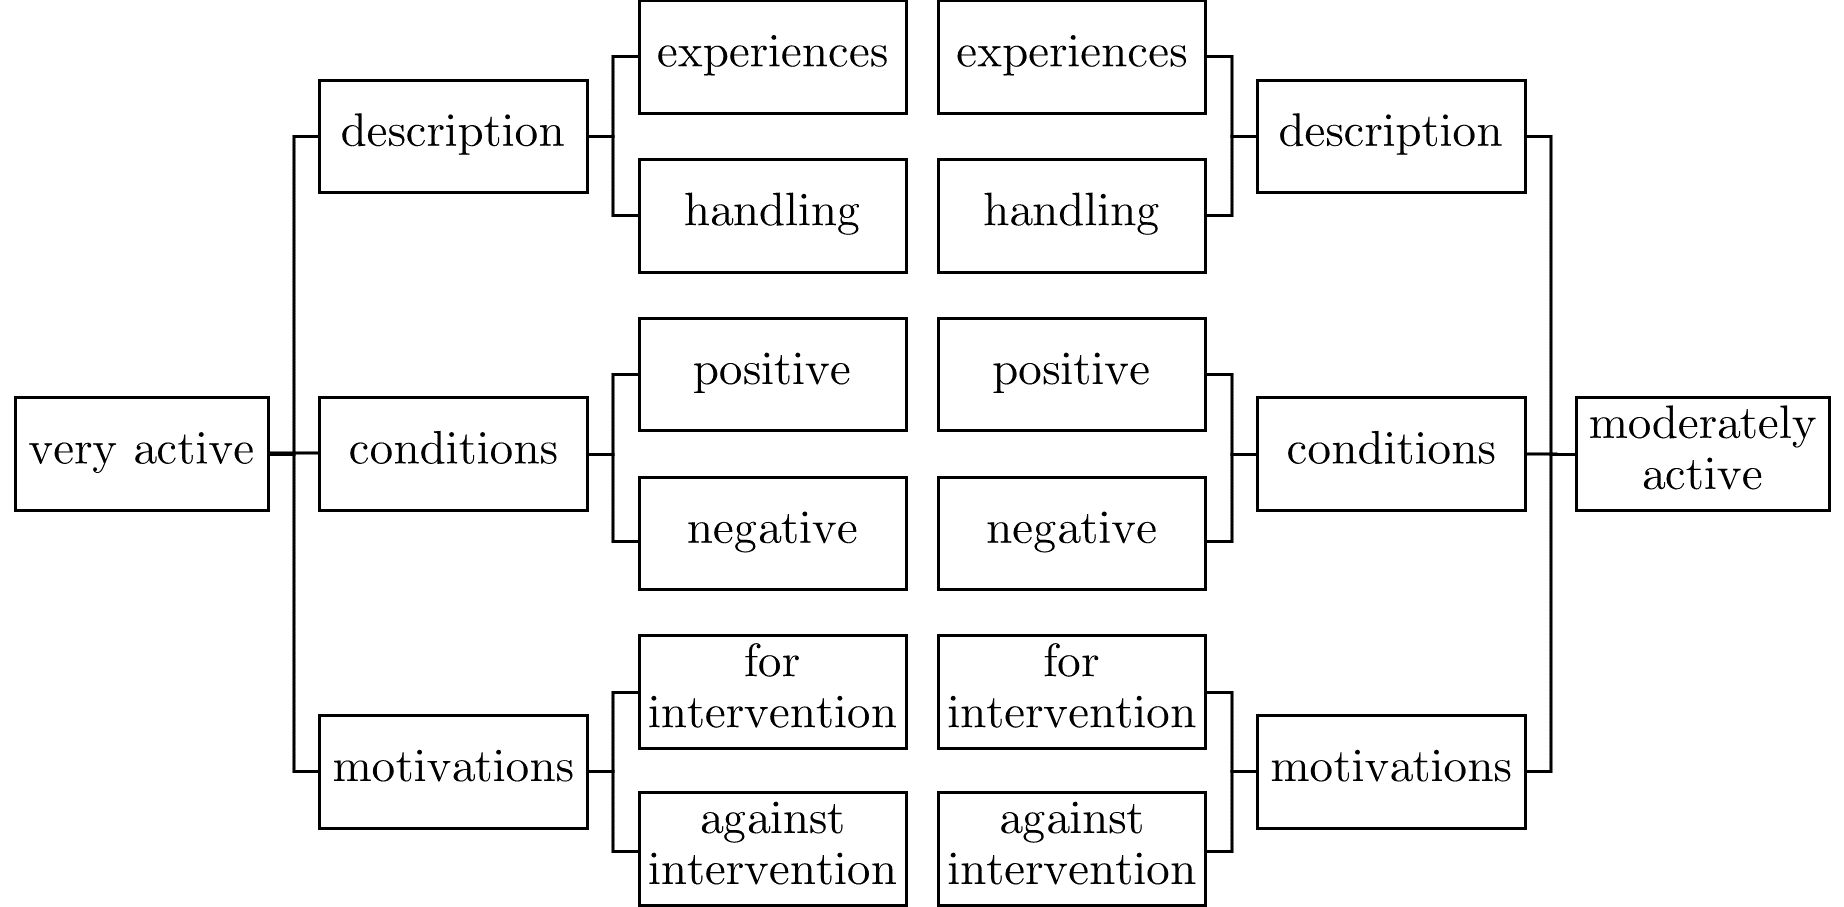
\includegraphics[width=1\linewidth]{../images/categorization} \caption{Overview of the final categorization}\label{fig:categorization}
\end{figure}

\hypertarget{results}{%
\section{Results}\label{results}}

As figure \ref{fig:categorization} shows, we contrasted the results of both groups for each category, (\emph{description}, \emph{conditions} and \emph{motivations}). As our research question focusses on predictors, only a quick overview will be given for the category \emph{description}.

For the sake of brevity, in the following sections these terms will be used:
\emph{Hater:} The perpetrator of the hate speech,
\emph{victim(s):} the recipient(s) or subject(s) of the hate speech, and
\emph{adversary victim(s):} victim(s) or subject(s) of hate speech that represent a group the participant politically or personally opposes.

\hypertarget{description-experiences-with-hate-speech-and-handling-hate-speech}{%
\subsection{Description: Experiences with Hate Speech and Handling Hate Speech}\label{description-experiences-with-hate-speech-and-handling-hate-speech}}

When describing their experiences with hate speech, both groups mention similar attributes of hate speech (e.g., the online \emph{spaces} where they have most often observed it). However, while four of the six very active participants report to have themselves been victims of hate speech, only one moderately active participants does so as well. There are also notable differences in the way participants of both groups handle hate speech: While participants in the moderately active group tend to look at hateful comments only for entertainment value or avoid looking at comments at all, many participants in the very active group actively seek out hate speech comments in order to fight it.

\hypertarget{conditions-when-to-engage-in-counter-speech}{%
\subsection{Conditions: When to Engage in Counter Speech}\label{conditions-when-to-engage-in-counter-speech}}

For a given situation, participants describe both conditions that make it more likely that they engage in counter speech ( \emph{positive conditions}) as well as conditions that make it less likely ( \emph{negative conditions}). As mentioned above, the participants in the moderately active group reported to only seldomely engage in counter speech at all, much less counter speech favoring \emph{adversary victims}, i.e., politically opposed users that are targetted by hate speech. Therefore, most of the conditions listed are to be understood as conditions for counter speech in general. The only exception is the subcategory \emph{positive conditions} for the very active group where a differentiation between counter speech in general and counter speech favoring \emph{adversary victims} was possible.

\hypertarget{positive-conditions-for-counter-speech-favoring-adversaries.}{%
\subsubsection{Positive Conditions for Counter Speech Favoring Adversaries.}\label{positive-conditions-for-counter-speech-favoring-adversaries.}}

When it comes defending people who they are politically opposed to, the following conditions emerged in the very active group: \textbf{1) Offenses against a \enquote{culture of discussion}}, i.e., the participant feels that the hater breaks the rules for a respectful debate, \textbf{2) offenses against the human dignity}, i.e., the participant feels that the hater debases the victim's human dignity, \textbf{3) properties of the victim}, e.g., the participants feels sympathy for the victim, and
\textbf{4) a personal connection to the topic discussed}.

\hypertarget{positive-conditions-for-counter-speech-in-general.}{%
\subsubsection{Positive Conditions for Counter Speech in General.}\label{positive-conditions-for-counter-speech-in-general.}}

\hypertarget{properties-of-the-hate-speech.}{%
\paragraph{Properties of the Hate Speech.}\label{properties-of-the-hate-speech.}}

Concerning the properties of the hate speech or the situation where the hate speech occurs, participants of both groups mention they are more likely to step in when they feel that their \textbf{1) counter speech is likely to have an impact}, e.g., there are not that many comments overall.
Additionally, participants of the very active group name the space as an important factor. They are more likely to step in when there is hate speech \textbf{2) outside of hater-dominated spaces}, e.g., not in a dedicated facebook group, or
\textbf{3) in a more private space}, e.g., in a personal chat group.

On the other side, participants of the moderately active group mention \textbf{4) calls to violence and threats} as well as
\textbf{5) doxxing}, i.e., finding and disseminating the victim's personal information,
as factors making counter speech more likely for them.

\hypertarget{properties-of-the-victim.}{%
\paragraph{Properties of the Victim.}\label{properties-of-the-victim.}}

Relating to the properties of the victim, both groups mention that they would be more likely to intervene if
\textbf{1) the victim is a private citizen} or if \textbf{2) they know the victim personally}, although that is more important in the moderately active group.
Additionaly, particicpants of the very active group would be more likely to engage in counter speech if \textbf{3) the victim is an activist}.

\hypertarget{personal-attributes.}{%
\paragraph{Personal Attributes.}\label{personal-attributes.}}

Participants of both group state that they are more likely to step in if they are \textbf{1) well informed about the topic of discussion}. Members of the very active group also name \textbf{2) free time and mental energy} as a condition. Some members of the moderately active group, on the other hand, describe \textbf{3) feeling frustrated and angry} or \textbf{4) having a personal connection} to the topic of discussion as a conductor for counter\textasciitilde speech.

\hypertarget{negative-conditions-for-counter-speech-in-general.}{%
\subsubsection{Negative Conditions for Counter Speech in General.}\label{negative-conditions-for-counter-speech-in-general.}}

Many of the \emph{negative conditions} mentioned in the group are merely negations of the \emph{positive conditions} already listed and will therefore not be reported again.

\hypertarget{properties-of-the-hate-speech.-1}{%
\paragraph{Properties of the Hate Speech.}\label{properties-of-the-hate-speech.-1}}

Members of both group state that they are less likely to engage in counter speech, when \textbf{1) both sides of the discussion engage in hate speech} or when
\textbf{2) the hate speech is entertaining to them}.

Additionally, participants of the very active group are less willing to intervene when they fear \textbf{3) personal risk to themselves}.

\hypertarget{properties-of-the-victim.-1}{%
\paragraph{Properties of the Victim.}\label{properties-of-the-victim.-1}}

Apart from the negatives to the \emph{positive conditions} already mentioned, one member of the very active group reports that they would be less likely to intervene if they suspect \textbf{the victim is eager to be seen as a victim by the public}.

\hypertarget{motivations-why-to-engage-in-counter-speech}{%
\subsection{Motivations: Why to Engage in Counter Speech}\label{motivations-why-to-engage-in-counter-speech}}

Just as with the conditions, the \emph{motivations} of the participants could also be categorized into \emph{motivations for intervention} and \emph{motivations against intervention}. In this context, \emph{motivations} relate to the participants' attitudes towards counter speech in general. By contrast, the \emph{conditions} listed above relate to specific situations.

\hypertarget{motivations-for-intervention.}{%
\subsubsection{Motivations for Intervention.}\label{motivations-for-intervention.}}

The \emph{motivations for intervention} can be further categorized into \emph{goals and values} and \emph{personal attributes and experiences}.

\hypertarget{goals-and-values.}{%
\paragraph{Goals and Values.}\label{goals-and-values.}}

Participants of both groups concede that while they might not be able to dissuade the hater from their destructive behavior, they still \textbf{1) hope to positively influence the audience}.
Members of the very active group are additionally motivated by the desire to
\textbf{2) fight disinformation},
\textbf{3) motivate critical thinking in other users},
\textbf{4) create a better culture of discussion in online spaces} and
\textbf{5) engage politically}.
Some of the very active participants describe viewing their counter speech activity as a form of activism.

Moderately active participants, on the other hand, worry that \emph{online hate might spark offline violence}.

\hypertarget{personal-attributes-and-experiences.}{%
\paragraph{Personal Attributes and Experiences.}\label{personal-attributes-and-experiences.}}

When it comes to their personal attributes and experiences that motivate them to engage in counter speech, participants of both groups mention
\textbf{1) a strong sense of justice } and
\textbf{2) a sense of responsibility}.

In addition, very active participants name
\textbf{1) enjoying debating},
\textbf{2) their own experiences with bullying and discrimination},
\textbf{3) enjoying self-promotion}, as well as
\textbf{4) being thanked and admired by others}, e.g., by site administrators,
as motivators.

\hypertarget{motivations-against-intervention.}{%
\subsubsection{Motivations against Intervention.}\label{motivations-against-intervention.}}

Members of both groups name one main motivation not to engage in counter speech: They think it is \textbf{1) not worth the effort}. On top of that, members of the very active group mainly mention \textbf{2) fatigue} with fighting hate speech in general as something that demotivates them from engaging in counter speech.

Among the moderately active participants, a considerable number more motivations are named:
\textbf{1) A general unwillingness to participate in online communication},
\textbf{2) a preference for alternative approaches to hate speech}, e.g.~blocking the perpetrator or even reporting them to the police,
\textbf{3) their perception of the chance to be successful as too small} and
\textbf{4) their own tendency to avoid reading comments at all}.

\hypertarget{discussion-and-conclusion}{%
\section{Discussion and Conclusion}\label{discussion-and-conclusion}}

Notably, a vast difference in engagement levels between the participants was found. While some would not engage in online discourse at all and consequently would not engage in counter speech either, others were hyperactive on social media, placing a lot of value on political discourse in online spaces. Participants in the latter group reported a much higher likelihood to engage in counter speech, be it on behalf of opponents or in general.

Overall, the relationship between the counter speaker and the victim which we focussed on in our research question (\emph{In social media discussions, what motivates users to engage in counter speech in support of political adversaries?}) seems to be less important than the willingness to engage in counter speech in general. While we collected and categorized the predictors for counter speech reported by our participants in \emph{conditions}, i.e., situational predictors, and \emph{motivations}, i.e., general predictors, there is only a small number of predictors from the subset \emph{conditions} strictly in answer to our research question:

Three basic motivations for users to engage in counter speech in support of political adversaries can be differentiated:
Firstly, the hater violates norms or values that are more important to the counter speaker than political affiliation.
Values named here were a \enquote{culture of discussion}, i.e., an implicit set of rules for a respectful debate, and \enquote{human dignity}.
These conditions tie somewhat into other findings about counter speakers placing high importance on morality \autocite{lambeStandingBullyingSocial2019,wilhelmGenderedMoralityBacklash2019}.
Interestingly, they also mirror the vision of the internet as a place for public deliberation \autocite{chenOnlineIncivilityPublic2017}.
Productive debates can only happen if all participants follow the rules, no matter which side they are on.
Secondly, counter speech is more likely if the participants feels sympathetic towards the victim.
This is similar to results from cyber-bullying research \autocite{lambeStandingBullyingSocial2019}. Thirdly, participants are more likely to intervene when they feel a personal connection to the topic of discussion. Both the second and the third motivation are limited in their generalizability. Sympathies are likely to wane the larger the distance on the political spectrum gets.
And in many occurences of hate speech, there will be no connection to a tangible discussion topic.

The other predictors we found refer to counter speech in general and therefore do not strictly answer the research question. However, as posited above, we did not observe the expected divide between people engaging in counter speech only for friends or members of their in-group and people engaging in counter speech for everyone---including adversaries. Rather, the divide was between people engaging in counter speech for everyone, regardless of political or group affiliation, and people not generally engaging in counter speech. As such, we feel that the \emph{motivations} of the very active group questioned also partly answer the question of what motivates counter speakers.

The most important \emph{motivations} we found were deep-seated moral convictions and a feeling of responsibility to uphold those convictions. This does not only match the findings by on the importance of morality by \textcite{wilhelmGenderedMoralityBacklash2019} and \textcite{lambeStandingBullyingSocial2019}. The acceptance of responsibility also matches the bystander model of intervention often used to describe bystander behavior in cyber-bullying incidents (e.g., \autocite{naabFlaggingUncivilUser2018}).
Moreover, the participants felt that online discourse is an important part of political participation \autocite{chenOnlineIncivilityPublic2017}.
Many of the active counter speakers we talked to saw their actions as a form of activism. One of their major goals was not to change the behavior of the people engaging in hate speech, but to positively influence the broader audience. This matches what \textcite{buergerCounterspeechLiteratureReview2019} call the contagion effect.

In conclusion, when looking at what motivates a person to regularly engage in counter speech, their relationship to the victim appears to be secondary. Of greater importance seems to be what part morality plays in that person's self-image and how willing they are to accept and defend online spaces as a place for public deliberation.

Finally, some limitations have to be noted: Firstly, although we tried to emphasize the relationship aspect (i.e., counter speech \emph{in favor of adversaries}) in our research design, stressing this emphasis during the focus groups proved challenging. Rather, participants tended to talk about their experiences with counter speech \emph{in general}. This holds especially true for the participants of the moderately active group, many of whom never had engaged in counter speech at all. Therefore, our results are not suitable to evaluate whether there are differences between predictors for counter speech \emph{in favor of adversaries} and counter speech \emph{in general}. Secondly, our sample was comparatively young, highly educated and politically left-aligned. It is entirely possible that other predictors not mentioned here are important with counter speakers who are, e.g., more politically right-leaning.
In any case, the predictors identified in this study should be further tested in a quantitative study.
Thirdly, the predictors identified in this study as well as most other studies listed in chapter \ref{predictors-for-counter-speech} are self-reported.
Conducting an experiment could shed light on whether or not these translate to actual defending behavior.

\hypertarget{acknowledgements}{%
\section*{Acknowledgements}\label{acknowledgements}}
\addcontentsline{toc}{section}{Acknowledgements}

We would like to thank Maximilian Geulen and Merten Wothge for their help in developing the research design as well as collecting the data.
This research was supported
by the Digital Society research program funded by the
Ministry of Culture and Science of the German State of North
Rhine-Westphalia. We would further like to thank the authors of the packages we have used.
We used the following packages to create this document: \texttt{knitr}~\autocite{R-knitr}, \texttt{tidyverse}~\autocite{R-tidyverse}, \texttt{rmdformats}~\autocite{R-rmdformats}, \texttt{kableExtra}~\autocite{R-kableExtra}, \texttt{rmdtemplates}~\autocite{R-rmdtemplates}, \texttt{citr}~\autocite{R-citr}.


%
% ---- Bibliography ----
%
% BibTeX users should specify bibliography style 'splncs04'.
% References will then be sorted and formatted in the correct style.
%
%\bibliographystyle{splncs04}
%\bibliography{bibliography,rpackages}
\printbibliography



\end{document}
